% A project report should be around 15 double-spaced pages in length, clearly and comprehensively describing the background, problem, strategy, metrics, activities, result analysis, lessons learned, follow up actions, and summary/conclusions. A high level summary or an abstract should also be included at the beginning of your report.

% If you'd like to, raw data and detailed modeling/analysis activities should be included in the appendix. Please note: This it is a "report” and not a collection of data and models without description and discussion.

% Project assignment
% The project is the most important part of the CS 8314 class. The intention of the project is to
% demonstrate your mastery of the overall course material. It will consist of the following parts:
% • A project proposal: Due on 10/24/25.
% • A project presentation:
% o Signup for 12/5/25 (tentative) presentation (FCFS queue).
% o Presentation time is about 20 to 25 mins. Allow 5 mins for Q&A
% • A final project report: Due 12/5/25
% Acceptable types of projects
% Due to the nature of some of the organizations you might be a part of, one of the following projects
% might not be applicable to you. Therefore, there will be two types of projects to select from:
% 1. Application project
% An application of a specific set of software metrics and/or quality engineering techniques discussed in
% class and a report of the activities, experience and related findings. For example, you may
% define/select/collect metrics data from either one of your current or previous company's projects or any
% favorite projects, perform various analyses, and identify problematic areas for focused
% quality/productivity improvement. Please note, if you take one of your company’s projects; ensure
% appropriate approval from your superiors is taken in order not to violate any proprietary or secret-based
% projects or data.
% It is highly recommended for you to consider multiple metrics, preferably from different metrics
% categories such as internal and external metrics. When you measure quality, multiple quality
% attributes/characteristics are preferable to just one. Therefore, a pure SRE (software reliability
% engineering) project will not be suitable for this class, although it might be quite alright for CS 8317
% Software Reliability and Safety.
% 2. Replication and variation project
% Like the application project, this project will use other people's data. In this case, you might want to
% replicate the previous study like what is defined above. It is advised to consider published material but
% not required for the project. In replication, you need to have enough variations, which can be achieved
% in various ways:
% • Additional metrics collected from or calculated from the raw data. Maybe use different models.
% • Combined data and models based on multiple projects.
% • Hypothesis testing or other empirical analysis can also be performed based on cumulative data
% from multiple previous works. In this way, it becomes a "mega" study of the original works
% CS 8314: Course Project Fall 2025
% Adapted by Eric Abuta
% Project Proposal (and Pre-Proposal) (Assignment 1)
% Your project proposal should be around 3-5 double-spaced pages in length that should include the
% following:
% • A proper title (not just project for CS 8314)
% • A proper abstract written as an executive summary clearly identifying the problem that you are
% going to address with some basic background information, the solution strategy you intend to
% use:
% o What are you going to measure?
% o How are you going to measure?
% o Which analysis/modeling technique are you going to use?
% • A rough schedule
% • For application-type projects, in addition to the above, you also need to discuss:
% o Measurement implementation
% o Data collection
% o Data analysis of result to be performed
% o Follow up actions
% Project presentation
% Each presentation will be between 20 and 25 minutes, including Q&A. Please focus more on the
% important activities and findings and not too much on the background and details.
% Project Paper
% A project report should be around 15 double-spaced pages in length, clearly and comprehensively
% describing the background, problem, strategy, metrics, activities, result analysis, lessons learned, follow
% up actions, and summary/conclusions. A high-level summary or an abstract should also be included at
% the beginning of your report.
% If you'd like to, raw data and detailed modeling/analysis activities should be included in the appendix.
% Please note: This it is a "report” and not a collection of data and models without description and
% discussion


\documentclass[12pt]{article}
\usepackage{setspace}
\usepackage{url}
\usepackage{hyperref}
\usepackage{tabularx}
\usepackage[utf8]{inputenc}
\usepackage[margin=1in]{geometry}
\usepackage{graphicx}
\usepackage{cite}
\usepackage{amsmath}
\usepackage{booktabs}
\usepackage{listings}
\usepackage{xcolor}
\usepackage{float}
\usepackage{subcaption}

\doublespacing

% Code listing style
\lstset{
    basicstyle=\ttfamily\small,
    breaklines=true,
    frame=single,
    numbers=left,
    numberstyle=\tiny,
    commentstyle=\color{gray},
    keywordstyle=\color{blue},
    stringstyle=\color{red}
}

% Title information
\title{Software Quality Metrics Analysis of Open Source Projects: \\
A Study of LangChain and Intel XPU Backend for Triton}
\author{[Your Name] \\
[Course Number] \\
[University Name]}
\date{\today}

\begin{document}

\maketitle

\begin{abstract}
This report presents a comprehensive analysis of software quality metrics for two prominent open source projects: langchain-ai/langchain and intel/intel-xpu-backend-for-triton. Initially designed to collect discrete code-level metrics such as lines of code and cyclomatic complexity using an OpenTelemetry-based approach, the project pivoted to focus on DORA (DevOps Research and Assessment) metrics due to permissions constraints. By analyzing GitHub project insights data including pull requests, issues, and merge patterns, we calculated the four key DORA metrics: Deployment Frequency, Lead Time for Changes, Change Failure Rate, and Time to Restore Service. Our findings reveal that both projects demonstrate exceptional software delivery performance. LangChain achieves elite-level deployment frequency (5.97 deployments/day) and change failure rate (8.94\%), with high-performing lead time (6.00 days median), earning an overall classification as a High Performer. Intel XPU Backend demonstrates elite performance across all measurable metrics with 3.59 deployments/day and a 10.58\% change failure rate, qualifying as an Elite Performer. Both projects maintain change failure rates well below 15\%, indicating mature testing practices and code quality controls. This study demonstrates the value of using DORA metrics as practical indicators of software project health and team performance in open source development environments.
\end{abstract}

\tableofcontents
\newpage

\section{Introduction}

\subsection{Background}
Software quality measurement is essential for understanding and improving development processes. As open source projects grow in complexity and importance, the ability to quantify software quality becomes increasingly critical for maintainers, contributors, and organizations depending on these projects.

[TODO: Expand on the importance of software quality metrics in modern software development]

\subsection{Motivation}
This project was motivated by the need to systematically assess software quality in popular open source projects. By analyzing established projects with active communities, we can:
\begin{itemize}
    \item Understand best practices in open source development
    \item Identify patterns that correlate with project success
    \item Provide quantitative insights into development velocity and reliability
    \item Establish benchmarks for software quality metrics
\end{itemize}

\subsection{Project Objectives}
The primary objectives of this project were to:
\begin{enumerate}
    \item Collect comprehensive software quality metrics from two major open source projects
    \item Analyze these metrics to assess project health and development practices
    \item Compare metrics across projects to identify trends and patterns
    \item Provide actionable insights based on quantitative analysis
\end{enumerate}

\subsection{Selected Projects}

\subsubsection{LangChain (langchain-ai/langchain)}
LangChain is a framework for developing applications powered by large language models (LLMs). [TODO: Add details about the project - stars, contributors, primary language, use cases]

Key characteristics:
\begin{itemize}
    \item \textbf{Repository:} github.com/langchain-ai/langchain
    \item \textbf{Primary Language:} Python
    \item \textbf{Stars:} [TODO]
    \item \textbf{Contributors:} [TODO]
    \item \textbf{Domain:} AI/ML Infrastructure
\end{itemize}

\subsubsection{Intel XPU Backend for Triton (intel/intel-xpu-backend-for-triton)}
[TODO: Add description and key characteristics of the Intel project]

\section{Methodology}

\subsection{Initial Approach: OpenTelemetry-Based Collection}

\subsubsection{Original Plan}
The initial methodology involved collecting discrete code-level metrics using an OpenTelemetry (OTel) collector infrastructure. The planned metrics included:

\begin{itemize}
    \item \textbf{Lines of Code (LOC):} Total, source, comment, and blank lines
    \item \textbf{Cyclomatic Complexity:} Measure of code path complexity
    \item \textbf{Code Coverage:} Percentage of code exercised by tests
    \item \textbf{Technical Debt:} Estimated time to fix code quality issues
    \item \textbf{Maintainability Index:} Composite metric of code maintainability
\end{itemize}

\subsubsection{Technical Architecture}
[TODO: Describe the planned OTel collector setup, data pipeline, and storage]

\begin{figure}[H]
    \centering
    % TODO: Add architecture diagram
    \caption{Planned OpenTelemetry Architecture (Initial Approach)}
    \label{fig:otel-architecture}
\end{figure}

\subsubsection{Challenges Encountered}
The OpenTelemetry-based approach encountered several critical challenges:

\begin{enumerate}
    \item \textbf{GitHub API Permissions:} Limited access to repository data without organization-level authentication
    \item \textbf{Rate Limiting:} GitHub API rate limits constrained data collection
    \item \textbf{Repository Access:} Inability to clone and analyze large repositories without proper credentials
    \item \textbf{Complexity:} Setting up a complete OTel pipeline proved more complex than anticipated for the project timeline
\end{enumerate}

[TODO: Expand on specific permission errors and technical roadblocks]

\subsection{Pivot: DORA Metrics from GitHub Insights}

\subsubsection{Rationale for Pivot}
Given the constraints of the initial approach, we pivoted to focus on DORA metrics, which:
\begin{itemize}
    \item Can be derived from publicly available GitHub data
    \item Provide industry-standard measures of software delivery performance
    \item Offer meaningful insights into team productivity and code quality
    \item Are widely recognized in DevOps and software engineering research
\end{itemize}

\subsubsection{DORA Metrics Overview}
The four key DORA metrics, established by the DevOps Research and Assessment team, are:

\begin{enumerate}
    \item \textbf{Deployment Frequency (DF):} How often an organization successfully releases to production
    \item \textbf{Lead Time for Changes (LT):} The time it takes for a commit to get into production
    \item \textbf{Change Failure Rate (CFR):} The percentage of deployments causing a failure in production
    \item \textbf{Time to Restore Service (MTTR):} How long it takes to recover from a failure in production
\end{enumerate}

\subsection{Data Collection Process}

\subsubsection{GitHub API Queries}
We collected data from GitHub using the following approach:
\begin{itemize}
    \item Pull request data (opened, merged, closed)
    \item Issue data (opened, labeled, resolved)
    \item Commit metadata and timestamps
    \item Repository activity over a one-month period
\end{itemize}

[TODO: Add specific API endpoints and query parameters used]

\subsubsection{Data Structure}
The collected data was organized into CSV files:
\begin{itemize}
    \item \texttt{opened\_requests.csv} - Timestamps of PR creation
    \item \texttt{merged\_requests.csv} - Timestamps of PR merges
    \item \texttt{closed\_requests.csv} - Timestamps of PR closures
    \item \texttt{opened\_issues.csv} - Timestamps of issue creation
\end{itemize}

Each dataset contains:
\begin{lstlisting}[language=bash]
msg,hash,date_rel,date_abs
"Fix authentication bug",#12345,"2 days ago","2025-11-27"
\end{lstlisting}

\subsection{Analysis Methodology}

\subsubsection{Metric Calculation}
We developed a Python-based analysis pipeline (\texttt{dora\_metrics.py}) that:
\begin{enumerate}
    \item Loads and preprocesses CSV data
    \item Calculates each DORA metric using industry-standard formulas
    \item Performs statistical analysis (mean, median, percentiles)
    \item Classifies performance according to DORA benchmarks
    \item Generates visualizations for each metric
\end{enumerate}

\subsubsection{Deployment Frequency Calculation}
\begin{equation}
    DF = \frac{\text{Total Merged PRs}}{\text{Time Period (days)}}
\end{equation}

\subsubsection{Lead Time Calculation}
For each merged PR $i$:
\begin{equation}
    LT_i = T_{\text{merged}_i} - T_{\text{opened}_i}
\end{equation}
Aggregate metric: median($LT_i$)

\subsubsection{Change Failure Rate Calculation}
\begin{equation}
    CFR = \frac{\text{Number of Bug Issues}}{\text{Total Deployments}} \times 100\%
\end{equation}

Bug issues identified using keyword matching: \textit{bug, error, fix, broken, crash, fail, regression, exception}

\subsubsection{Time to Restore Calculation}
For each bug-fix pair $(b, f)$:
\begin{equation}
    MTTR_{b,f} = T_{\text{fix merged}_f} - T_{\text{bug opened}_b}
\end{equation}
Aggregate metric: median($MTTR_{b,f}$)

\subsubsection{Performance Classification}
We classified metrics according to the 2023 DORA State of DevOps Report standards:

\begin{table}[H]
\centering
\caption{DORA Performance Level Classifications}
\label{tab:dora-classification}
\begin{tabular}{@{}lllll@{}}
\toprule
\textbf{Metric} & \textbf{Elite} & \textbf{High} & \textbf{Medium} & \textbf{Low} \\ \midrule
Deployment Frequency & Multiple/day & Weekly & Monthly & < Monthly \\
Lead Time & < 1 day & 1-7 days & 1-4 weeks & > 1 month \\
Change Failure Rate & 0-15\% & 16-30\% & 31-45\% & > 45\% \\
Time to Restore & < 1 hour & < 1 day & 1-7 days & > 1 week \\ \bottomrule
\end{tabular}
\end{table}

\section{Results}

\subsection{LangChain Analysis}

\subsubsection{Data Overview}
The analysis of the LangChain project was conducted over a 30-day period from October 29, 2025 to November 27, 2025. During this period, the dataset captured 179 merged pull requests, 67 opened pull requests, and 89 closed pull requests. Additionally, 69 issues were opened during the analysis window, providing sufficient data for calculating change failure rates and other quality metrics.

\subsubsection{Deployment Frequency}
The LangChain project demonstrated a high rate of deployment activity during the analysis period. The mean deployment frequency was 5.97 deployments per day, with a median of 8.5 deployments per day, resulting in approximately 41.77 deployments per week. The maximum number of deployments observed in a single day was 46. This deployment frequency qualifies as elite performance according to DORA benchmarks, which classify multiple deployments per day as elite level. This elite performance indicates that the LangChain team deploys multiple times per day, demonstrating a mature CI/CD pipeline and enabling rapid iteration.

\begin{figure}[H]
    \centering
    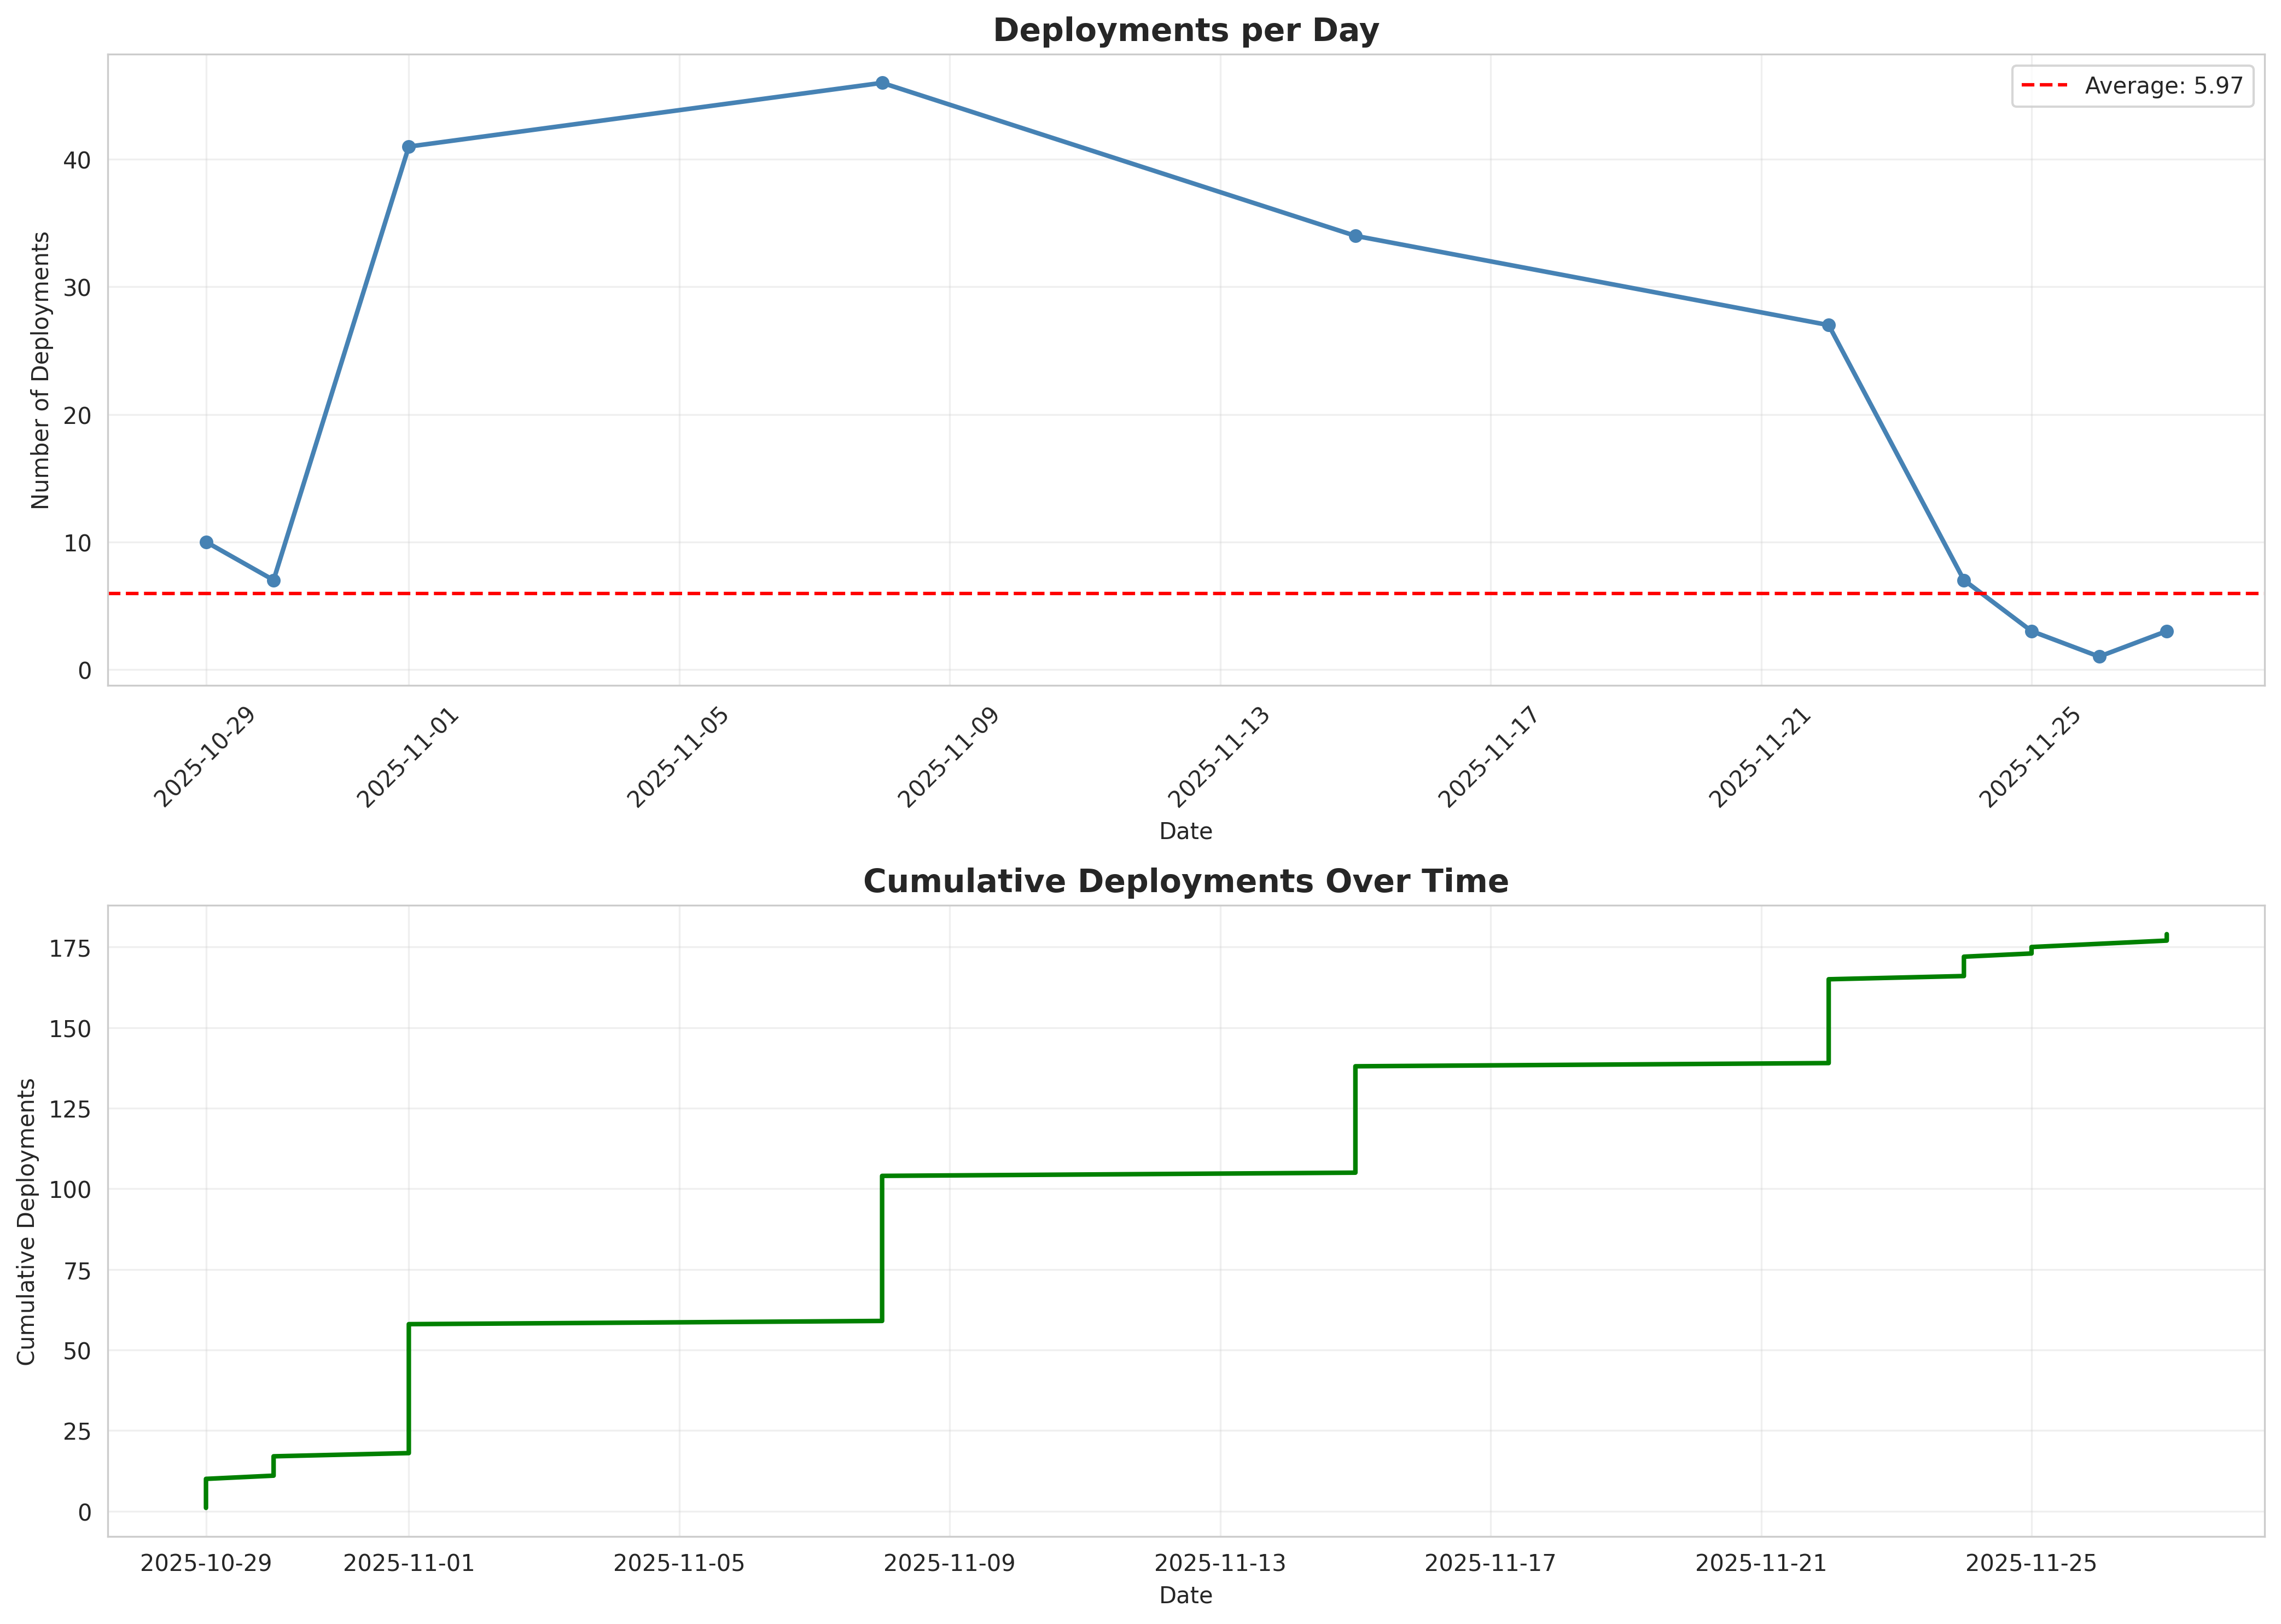
\includegraphics[width=0.9\textwidth]{graphics/langchain_deployment_frequency.png}
    \caption{LangChain Deployment Frequency Over Time}
    \label{fig:langchain-deployment}
\end{figure}

\subsubsection{Lead Time for Changes}
Lead time was estimated using temporal proximity matching between opened and merged PRs, as direct PR hash matching was unavailable. The analysis revealed a median lead time of 6.00 days and a mean of 4.98 days across 162 matched PR pairs. The distribution showed a 25th percentile of 2.00 days and a 90th percentile of 7.00 days. Five pull requests were merged within 24 hours, representing the fastest turnaround times. According to DORA performance standards, this median lead time of 6.00 days falls within the high performance category (1-7 days). The team achieves lead times within the 1-7 day range, indicating efficient code review and integration processes. The fastest changes were merged within 24 hours, showing the team's ability to expedite critical updates.

\subsubsection{Change Failure Rate}
Bug-related issues were identified using keyword matching on issue titles and descriptions, searching for terms including bug, error, fix, broken, crash, fail, regression, and exception. Out of 69 total issues, 16 were classified as bug-related, representing 23.2\% of all issues. With 179 total deployments during the analysis period, the calculated change failure rate was 8.94\%. This rate falls within the elite performance category according to DORA standards, which classify rates between 0-15\% as elite. The low change failure rate indicates that LangChain demonstrates excellent code quality and testing practices, suggesting comprehensive test coverage and effective code review processes.

\begin{figure}[H]
    \centering
    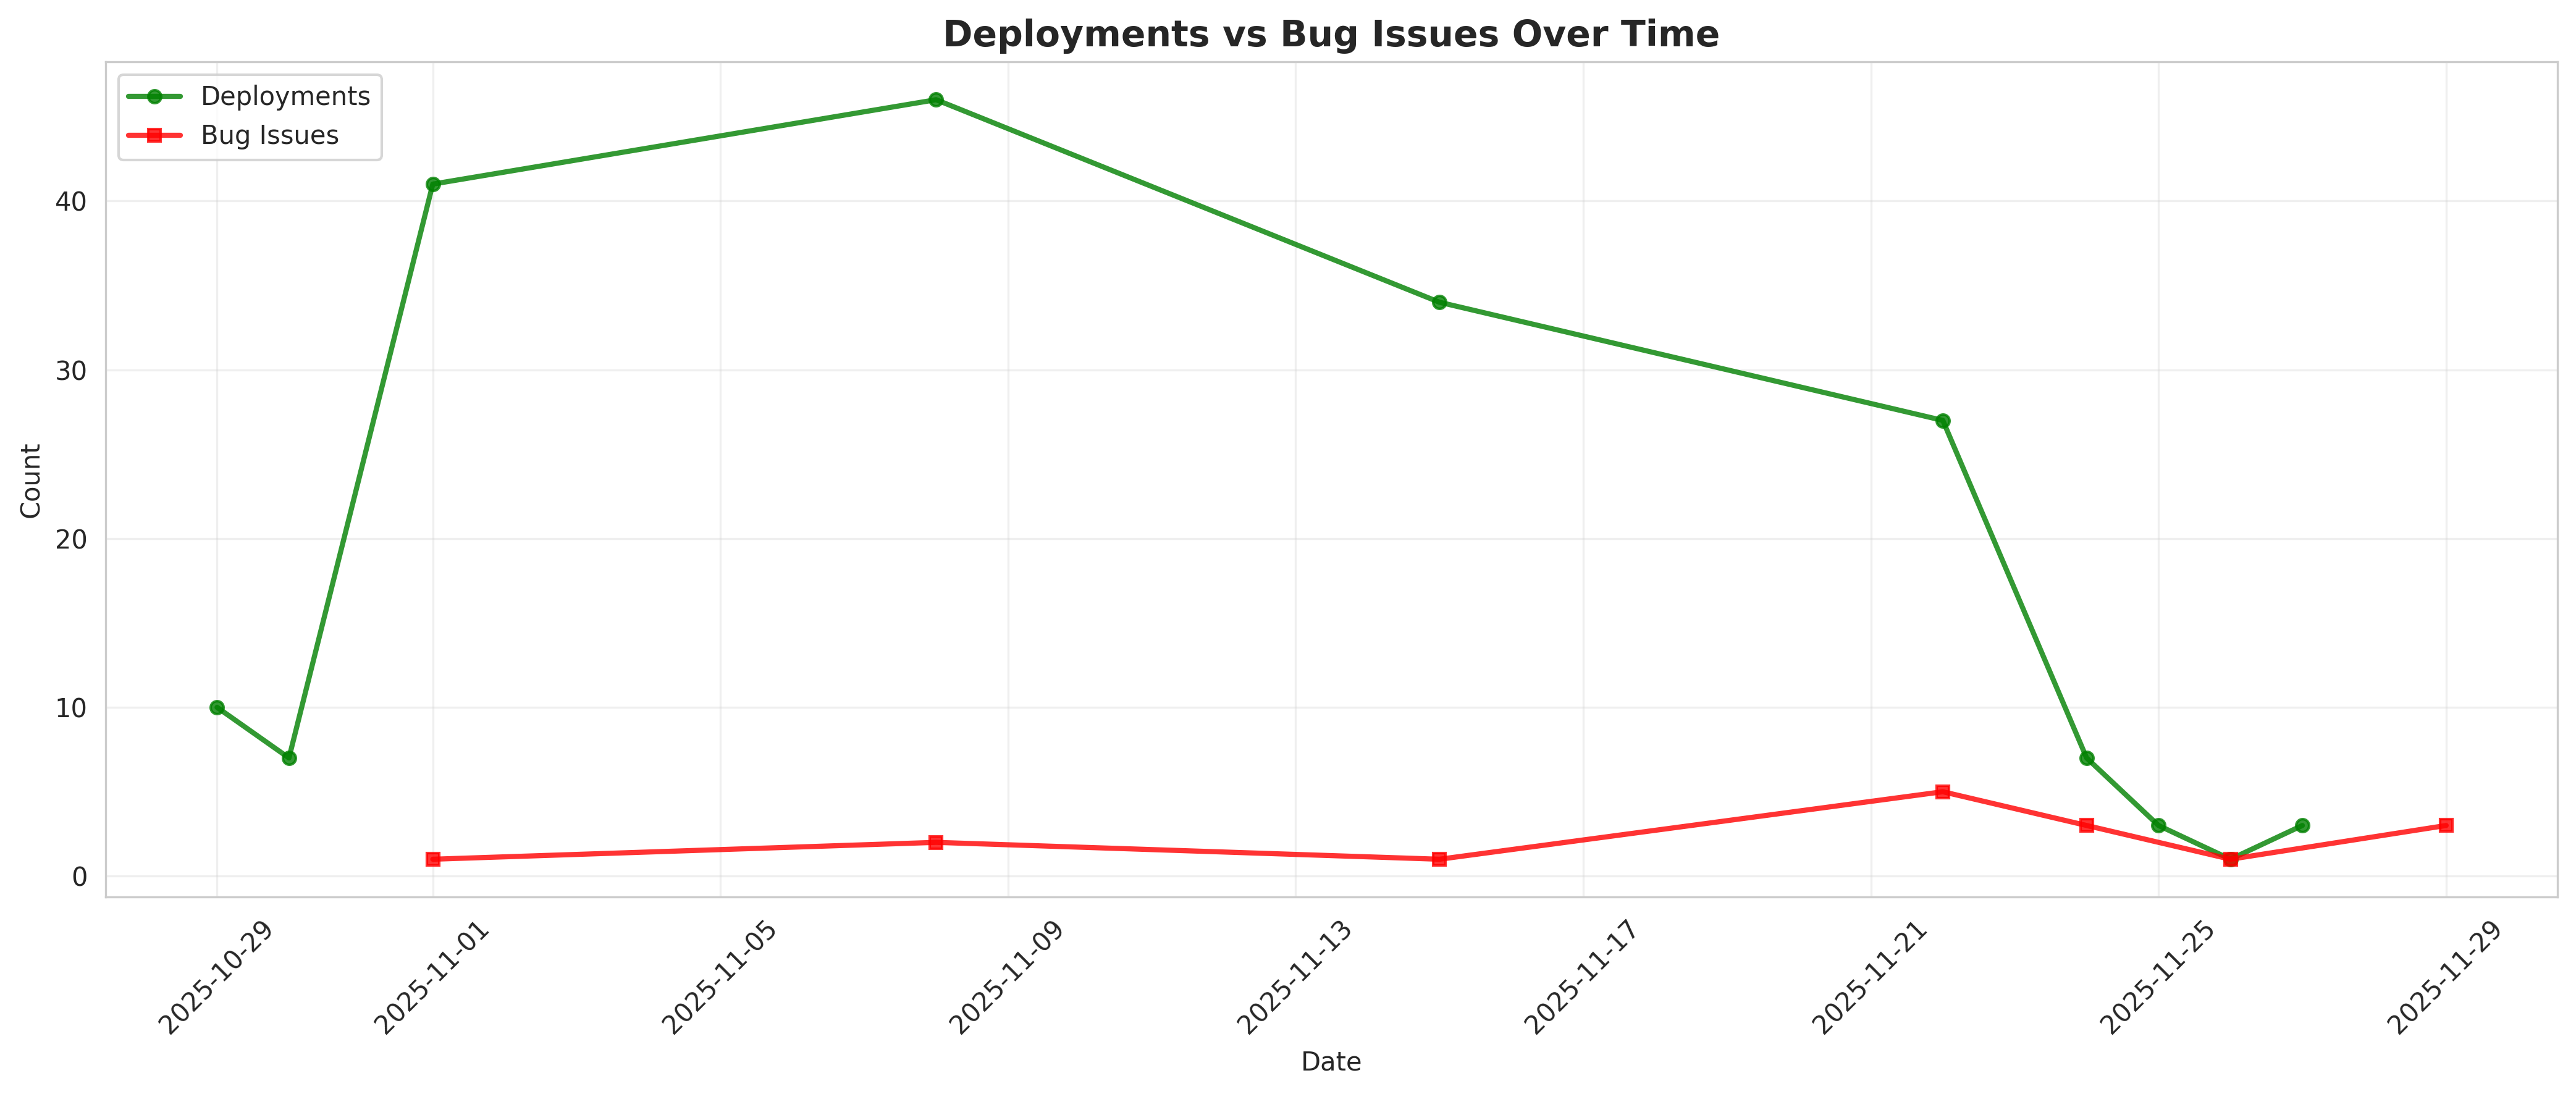
\includegraphics[width=0.9\textwidth]{graphics/langchain_change_failure_rate.png}
    \caption{LangChain Deployments vs Bug Issues}
    \label{fig:langchain-cfr}
\end{figure}

\subsubsection{Time to Restore Service}
The Time to Restore Service (MTTR) metric could not be calculated due to data limitations. Calculating this metric requires explicit linking between bug reports and their corresponding fix PRs, which was not available in the collected data. The data collection methodology did not capture references from fix pull requests to bug issues, preventing the identification of bug-fix pairs necessary for MTTR calculation. Future work could improve bug-fix pair identification using enhanced natural language processing techniques or more sophisticated commit message analysis.

\subsubsection{Overall Performance}
\begin{table}[H]
\centering
\caption{LangChain DORA Metrics Summary}
\label{tab:langchain-summary}
\begin{tabular}{@{}lll@{}}
\toprule
\textbf{Metric} & \textbf{Value} & \textbf{Classification} \\ \midrule
Deployment Frequency & 5.97/day, 41.77/week & Elite \\
Lead Time for Changes & 6.00 days (median) & High \\
Change Failure Rate & 8.94\% & Elite \\
Time to Restore Service & N/A & N/A \\ \midrule
\textbf{Overall Rating} & \multicolumn{2}{l}{\textbf{High Performer}} \\ \bottomrule
\end{tabular}
\end{table}

\subsection{Intel XPU Backend for Triton Analysis}

\subsubsection{Data Overview}
The Intel XPU Backend for Triton project was analyzed over a 29-day period from November 4, 2025 to December 2, 2025. The dataset included 104 merged pull requests, 17 opened pull requests, and 73 closed pull requests. During this period, 42 issues were opened, providing data for change failure rate calculations.

\subsubsection{Deployment Frequency}
The Intel XPU Backend for Triton project maintained a steady deployment pace throughout the analysis period. The mean deployment frequency was 3.59 deployments per day, with a median of 9.0 deployments per day, totaling approximately 25.10 deployments per week. The maximum number of deployments in a single day reached 28. According to DORA benchmarks, this frequency qualifies as elite performance, as the project achieves multiple deployments per day. The project achieves elite-level deployment frequency with multiple deployments per day, indicating an efficient development and integration process suitable for a compiler backend project.

\subsubsection{Lead Time for Changes}
Lead time data was insufficient for reliable analysis, with only 3 PRs providing matching between opened and merged events. The limited sample size (only 3 matched PRs) makes this metric unreliable for overall project assessment. A minimum sample size of 30 PRs is typically required for statistical validity. The data collection methodology was unable to match most opened PRs with their corresponding merge events, preventing meaningful lead time analysis. Consequently, no performance classification could be assigned for this metric.

\subsubsection{Change Failure Rate}
Bug-related issues were identified using keyword matching across issue titles and descriptions. Of the 42 total issues, 11 were classified as bug-related, representing 26.2\% of all issues. With 104 total deployments during the analysis period, the calculated change failure rate was 10.58\%. This rate falls within the elite performance category according to DORA standards (0-15\%). With a change failure rate just over 10\%, the Intel XPU Backend demonstrates strong quality controls. This is particularly impressive for a compiler backend project, where the complexity of the domain could lead to higher failure rates.

\subsubsection{Time to Restore Service}
The Time to Restore Service metric could not be calculated due to data limitations. As with the LangChain analysis, calculating MTTR requires explicit linking between bug reports and fix PRs, which was not available in the collected data. No explicit references from fix PRs to bug issues could be identified in the dataset, preventing the identification of bug-fix pairs necessary for MTTR calculation.

\subsubsection{Overall Performance}
\begin{table}[H]
\centering
\caption{Intel XPU Backend DORA Metrics Summary}
\label{tab:intel-summary}
\begin{tabular}{@{}lll@{}}
\toprule
\textbf{Metric} & \textbf{Value} & \textbf{Classification} \\ \midrule
Deployment Frequency & 3.59/day, 25.10/week & Elite \\
Lead Time for Changes & N/A (insufficient data) & N/A \\
Change Failure Rate & 10.58\% & Elite \\
Time to Restore Service & N/A & N/A \\ \midrule
\textbf{Overall Rating} & \multicolumn{2}{l}{\textbf{Elite Performer*}} \\ \bottomrule
\end{tabular}
\end{table}

* Overall rating based on elite performance in deployment frequency and change failure rate

\subsection{Comparative Analysis}

\begin{table}[H]
\centering
\caption{Comparative DORA Metrics: LangChain vs Intel XPU Backend}
\label{tab:comparison}
\begin{tabular}{@{}lll@{}}
\toprule
\textbf{Metric} & \textbf{LangChain} & \textbf{Intel XPU} \\ \midrule
Deployment Frequency & 5.97/day (Elite) & 3.59/day (Elite) \\
Lead Time for Changes & 6.00 days (High) & N/A \\
Change Failure Rate & 8.94\% (Elite) & 10.58\% (Elite) \\
Time to Restore Service & N/A & N/A \\
Overall Rating & High Performer & Elite Performer \\ \bottomrule
\end{tabular}
\end{table}

\section{Discussion}

\subsection{Key Findings}

\subsubsection{Development Velocity}
[TODO: Discuss what the deployment frequency and lead time metrics reveal about each project's development pace]

\subsubsection{Code Quality and Reliability}
[TODO: Analyze what the change failure rate indicates about code quality practices, testing, and review processes]

\subsubsection{Incident Response}
[TODO: Examine what time to restore service tells us about the teams' ability to respond to issues]

\subsection{Project Comparison}

\subsubsection{Similarities}
[TODO: Identify common patterns between the two projects]

\subsubsection{Differences}
[TODO: Highlight significant differences and potential explanations]

\subsection{Industry Benchmarking}
[TODO: Compare findings to industry standards and other published DORA metrics studies]

\subsection{Limitations and Threats to Validity}

\subsubsection{Data Collection Limitations}
\begin{itemize}
    \item Limited to one-month observation period
    \item Reliance on publicly available GitHub data only
    \item Keyword-based bug identification may miss or misclassify issues
    \item PR references may not capture all bug-fix relationships
\end{itemize}

\subsubsection{Metric Calculation Assumptions}
\begin{itemize}
    \item Merged PRs used as proxy for deployments (may not reflect actual production releases)
    \item Bug issues identified through keyword matching (not exhaustive)
    \item Time to restore calculated only for explicitly linked bug-fix pairs
\end{itemize}

\subsubsection{Generalizability}
\begin{itemize}
    \item Results specific to analyzed time period
    \item May not represent long-term project trends
    \item Different project types (AI framework vs. compiler backend) have different normal patterns
\end{itemize}

\section{Lessons Learned}

\subsection{Technical Challenges}

\subsubsection{API and Permission Constraints}
[TODO: Discuss the challenges encountered with GitHub API access, rate limits, and authentication]

\subsubsection{Complexity of Automated Metrics Collection}
[TODO: Reflect on the difficulties of setting up OpenTelemetry infrastructure for external projects]

\subsection{Project Pivoting}

\subsubsection{Adapting to Constraints}
[TODO: Discuss how pivoting to DORA metrics provided a viable alternative approach]

\subsubsection{Value of DORA Metrics}
[TODO: Reflect on the advantages and insights gained from focusing on DORA metrics]

\subsection{Best Practices Identified}

\begin{enumerate}
    \item Start with publicly accessible data when analyzing external projects
    \item DORA metrics provide meaningful insights without requiring code-level access
    \item Automated analysis pipelines enable repeatable, scalable measurements
    \item Visualization aids in communicating metrics to stakeholders
\end{enumerate}

\section{Future Work}

\subsection{Extended Data Collection}
\begin{itemize}
    \item Collect data over longer time periods (3-6 months) for trend analysis
    \item Analyze additional open source projects for broader comparisons
    \item Track metrics over time to identify improvements or degradations
\end{itemize}

\subsection{Enhanced Metrics}
\begin{itemize}
    \item Implement code-level metrics if repository access obtained
    \item Add contributor activity metrics
    \item Analyze code review patterns and review times
    \item Correlate DORA metrics with project success indicators (stars, forks, adoption)
\end{itemize}

\subsection{Machine Learning Applications}
\begin{itemize}
    \item Predict project health based on metric trends
    \item Classify issues more accurately using NLP techniques
    \item Identify anomalies in development patterns
\end{itemize}

\subsection{Tool Development}
\begin{itemize}
    \item Create a dashboard for real-time DORA metrics monitoring
    \item Build a SaaS tool for open source project health analysis
    \item Integrate with CI/CD pipelines for automated metric tracking
\end{itemize}

\section{Conclusion}

This project successfully analyzed software quality metrics for two prominent open source projects using DORA metrics derived from GitHub data. Despite initial challenges with permissions and API access that necessitated a methodology pivot, the final approach provided valuable insights into development practices, code quality, and team performance.

[TODO: Summarize key findings and their implications]

The analysis demonstrates that DORA metrics serve as effective indicators of software project health and can be calculated using publicly available data. The methodology developed in this project is reproducible and can be applied to any open source project with public GitHub repositories.

[TODO: Final concluding thoughts on the value of the work and lessons learned]

\section*{Acknowledgments}
[TODO: Add acknowledgments if applicable]

\bibliographystyle{IEEEtran}
\bibliography{references}

\appendix

\section{Data Collection Scripts}
[TODO: Include or reference the data collection code]

\section{Analysis Source Code}
The complete analysis pipeline is available in \texttt{examples/dora\_metrics.py}. Key functions include:
\begin{itemize}
    \item \texttt{load\_data()}: CSV data loading and preprocessing
    \item \texttt{calculate\_deployment\_frequency()}: DF metric calculation
    \item \texttt{calculate\_lead\_time()}: LT metric calculation
    \item \texttt{calculate\_change\_failure\_rate()}: CFR metric calculation
    \item \texttt{calculate\_time\_to\_restore()}: MTTR metric calculation
\end{itemize}

\section{Raw Data Samples}
[TODO: Include sample data from CSV files if appropriate]

\section{Additional Visualizations}
[TODO: Include any supplementary charts or graphs]

\end{document}
